% Created by tikzDevice version 0.12 on 2020-02-07 10:57:54
% !TEX encoding = UTF-8 Unicode
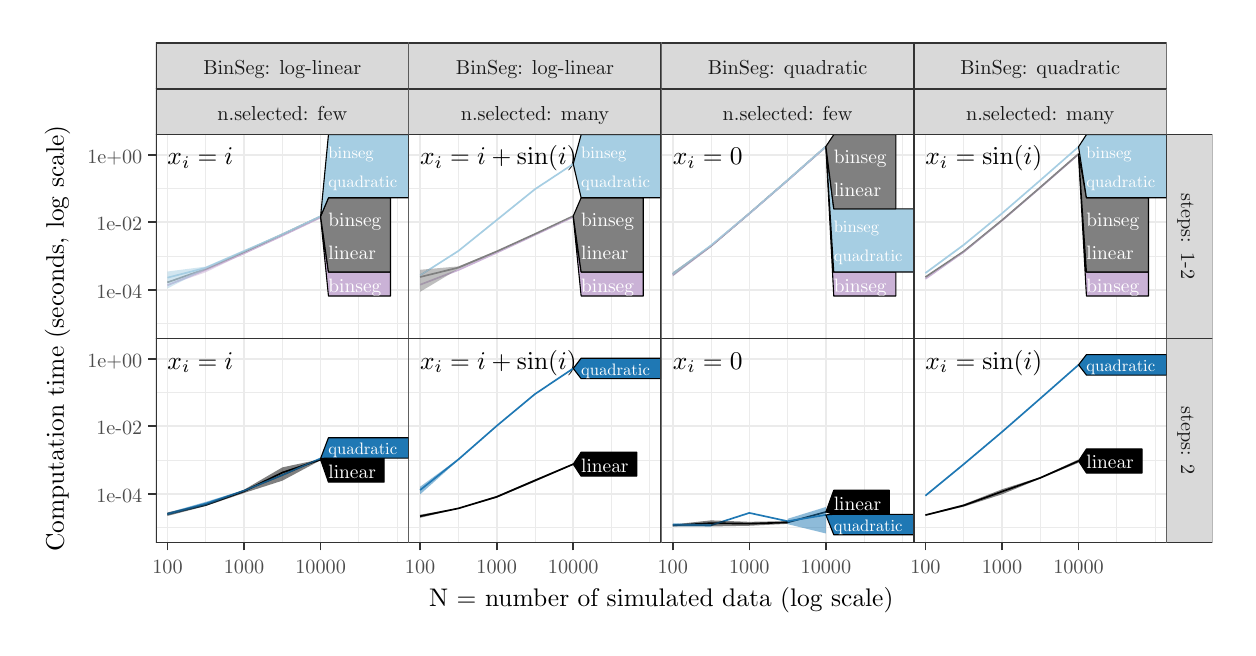
\begin{tikzpicture}[x=1pt,y=1pt]
\definecolor{fillColor}{RGB}{255,255,255}
\path[use as bounding box,fill=fillColor,fill opacity=0.00] (0,0) rectangle (433.62,216.81);
\begin{scope}
\path[clip] (  0.00,  0.00) rectangle (433.62,216.81);
\definecolor{drawColor}{RGB}{255,255,255}
\definecolor{fillColor}{RGB}{255,255,255}

\path[draw=drawColor,line width= 0.6pt,line join=round,line cap=round,fill=fillColor] (  0.00,  0.00) rectangle (433.62,216.81);
\end{scope}
\begin{scope}
\path[clip] ( 46.36,104.43) rectangle (137.66,178.17);
\definecolor{fillColor}{RGB}{255,255,255}

\path[fill=fillColor] ( 46.36,104.43) rectangle (137.66,178.17);
\definecolor{drawColor}{gray}{0.92}

\path[draw=drawColor,line width= 0.3pt,line join=round] ( 46.36,109.94) --
	(137.66,109.94);

\path[draw=drawColor,line width= 0.3pt,line join=round] ( 46.36,134.31) --
	(137.66,134.31);

\path[draw=drawColor,line width= 0.3pt,line join=round] ( 46.36,158.68) --
	(137.66,158.68);

\path[draw=drawColor,line width= 0.3pt,line join=round] ( 64.35,104.43) --
	( 64.35,178.17);

\path[draw=drawColor,line width= 0.3pt,line join=round] ( 92.01,104.43) --
	( 92.01,178.17);

\path[draw=drawColor,line width= 0.3pt,line join=round] (119.68,104.43) --
	(119.68,178.17);

\path[draw=drawColor,line width= 0.3pt,line join=round] (133.51,104.43) --
	(133.51,178.17);

\path[draw=drawColor,line width= 0.6pt,line join=round] ( 46.36,122.13) --
	(137.66,122.13);

\path[draw=drawColor,line width= 0.6pt,line join=round] ( 46.36,146.50) --
	(137.66,146.50);

\path[draw=drawColor,line width= 0.6pt,line join=round] ( 46.36,170.87) --
	(137.66,170.87);

\path[draw=drawColor,line width= 0.6pt,line join=round] ( 50.51,104.43) --
	( 50.51,178.17);

\path[draw=drawColor,line width= 0.6pt,line join=round] ( 78.18,104.43) --
	( 78.18,178.17);

\path[draw=drawColor,line width= 0.6pt,line join=round] (105.85,104.43) --
	(105.85,178.17);
\definecolor{drawColor}{RGB}{0,0,0}

\node[text=drawColor,anchor=base west,inner sep=0pt, outer sep=0pt, scale=  0.92] at ( 50.51,167.21) {$x_i = i$};
\definecolor{drawColor}{RGB}{202,178,214}

\path[draw=drawColor,line width= 0.6pt,line join=round] ( 50.51,123.75) --
	( 64.35,129.32) --
	( 78.18,135.26) --
	( 92.01,141.64) --
	(105.85,148.23);
\definecolor{drawColor}{gray}{0.50}

\path[draw=drawColor,line width= 0.6pt,line join=round] ( 50.51,124.78) --
	( 64.35,129.63) --
	( 78.18,135.78) --
	( 92.01,142.11) --
	(105.85,148.60);
\definecolor{drawColor}{RGB}{166,206,227}

\path[draw=drawColor,line width= 0.6pt,line join=round] ( 50.51,126.47) --
	( 64.35,130.03) --
	( 78.18,136.04) --
	( 92.01,142.14) --
	(105.85,148.64);
\definecolor{fillColor}{RGB}{202,178,214}

\path[fill=fillColor,fill opacity=0.50] ( 50.51,123.88) --
	( 64.35,130.10) --
	( 78.18,135.41) --
	( 92.01,141.68) --
	(105.85,148.42) --
	(105.85,148.04) --
	( 92.01,141.60) --
	( 78.18,135.10) --
	( 64.35,128.41) --
	( 50.51,123.62) --
	cycle;
\definecolor{fillColor}{RGB}{127,127,127}

\path[fill=fillColor,fill opacity=0.50] ( 50.51,124.93) --
	( 64.35,129.70) --
	( 78.18,136.00) --
	( 92.01,142.16) --
	(105.85,148.62) --
	(105.85,148.57) --
	( 92.01,142.06) --
	( 78.18,135.55) --
	( 64.35,129.55) --
	( 50.51,124.63) --
	cycle;
\definecolor{fillColor}{RGB}{166,206,227}

\path[fill=fillColor,fill opacity=0.50] ( 50.51,128.69) --
	( 64.35,130.47) --
	( 78.18,136.46) --
	( 92.01,142.17) --
	(105.85,148.69) --
	(105.85,148.58) --
	( 92.01,142.11) --
	( 78.18,135.58) --
	( 64.35,129.56) --
	( 50.51,122.59) --
	cycle;
\end{scope}
\begin{scope}
\path[clip] ( 46.36,104.43) rectangle (137.66,178.17);
\definecolor{drawColor}{RGB}{0,0,0}
\definecolor{fillColor}{RGB}{202,178,214}

\path[draw=drawColor,line width= 0.4pt,line join=round,line cap=round,fill=fillColor] (105.85,148.23) --
	(108.69,128.52) --
	(131.12,128.52) --
	(131.12,119.84) --
	(108.69,119.84) --
	cycle;
\definecolor{fillColor}{gray}{0.50}

\path[draw=drawColor,line width= 0.4pt,line join=round,line cap=round,fill=fillColor] (105.85,148.60) --
	(108.69,155.34) --
	(131.12,155.34) --
	(131.12,128.52) --
	(108.69,128.52) --
	cycle;
\definecolor{fillColor}{RGB}{166,206,227}

\path[draw=drawColor,line width= 0.4pt,line join=round,line cap=round,fill=fillColor] (105.85,148.64) --
	(108.69,178.17) --
	(137.66,178.17) --
	(137.66,155.34) --
	(108.69,155.34) --
	cycle;
\definecolor{drawColor}{RGB}{255,255,255}

\node[text=drawColor,anchor=base west,inner sep=0pt, outer sep=0pt, scale=  0.70] at (108.69,121.28) {binseg};

\node[text=drawColor,anchor=base west,inner sep=0pt, outer sep=0pt, scale=  0.70] at (108.69,145.08) {binseg};

\node[text=drawColor,anchor=base west,inner sep=0pt, outer sep=0pt, scale=  0.70] at (108.69,132.99) {linear};

\node[text=drawColor,anchor=base west,inner sep=0pt, outer sep=0pt, scale=  0.60] at (108.69,169.44) {binseg};

\node[text=drawColor,anchor=base west,inner sep=0pt, outer sep=0pt, scale=  0.60] at (108.69,159.14) {quadratic};
\definecolor{drawColor}{gray}{0.20}

\path[draw=drawColor,line width= 0.6pt,line join=round,line cap=round] ( 46.36,104.43) rectangle (137.66,178.17);
\end{scope}
\begin{scope}
\path[clip] ( 46.36, 30.69) rectangle (137.66,104.43);
\definecolor{fillColor}{RGB}{255,255,255}

\path[fill=fillColor] ( 46.36, 30.69) rectangle (137.66,104.43);
\definecolor{drawColor}{gray}{0.92}

\path[draw=drawColor,line width= 0.3pt,line join=round] ( 46.36, 36.20) --
	(137.66, 36.20);

\path[draw=drawColor,line width= 0.3pt,line join=round] ( 46.36, 60.57) --
	(137.66, 60.57);

\path[draw=drawColor,line width= 0.3pt,line join=round] ( 46.36, 84.94) --
	(137.66, 84.94);

\path[draw=drawColor,line width= 0.3pt,line join=round] ( 64.35, 30.69) --
	( 64.35,104.43);

\path[draw=drawColor,line width= 0.3pt,line join=round] ( 92.01, 30.69) --
	( 92.01,104.43);

\path[draw=drawColor,line width= 0.3pt,line join=round] (119.68, 30.69) --
	(119.68,104.43);

\path[draw=drawColor,line width= 0.3pt,line join=round] (133.51, 30.69) --
	(133.51,104.43);

\path[draw=drawColor,line width= 0.6pt,line join=round] ( 46.36, 48.39) --
	(137.66, 48.39);

\path[draw=drawColor,line width= 0.6pt,line join=round] ( 46.36, 72.76) --
	(137.66, 72.76);

\path[draw=drawColor,line width= 0.6pt,line join=round] ( 46.36, 97.13) --
	(137.66, 97.13);

\path[draw=drawColor,line width= 0.6pt,line join=round] ( 50.51, 30.69) --
	( 50.51,104.43);

\path[draw=drawColor,line width= 0.6pt,line join=round] ( 78.18, 30.69) --
	( 78.18,104.43);

\path[draw=drawColor,line width= 0.6pt,line join=round] (105.85, 30.69) --
	(105.85,104.43);
\definecolor{drawColor}{RGB}{0,0,0}

\node[text=drawColor,anchor=base west,inner sep=0pt, outer sep=0pt, scale=  0.92] at ( 50.51, 93.47) {$x_i = i$};

\path[draw=drawColor,line width= 0.6pt,line join=round] ( 50.51, 41.05) --
	( 64.35, 44.34) --
	( 78.18, 49.28) --
	( 92.01, 56.04) --
	(105.85, 60.70);
\definecolor{drawColor}{RGB}{31,120,180}

\path[draw=drawColor,line width= 0.6pt,line join=round] ( 50.51, 41.11) --
	( 64.35, 44.85) --
	( 78.18, 49.50) --
	( 92.01, 55.14) --
	(105.85, 61.16);
\definecolor{fillColor}{RGB}{0,0,0}

\path[fill=fillColor,fill opacity=0.50] ( 50.51, 41.64) --
	( 64.35, 44.70) --
	( 78.18, 49.84) --
	( 92.01, 57.91) --
	(105.85, 60.87) --
	(105.85, 60.52) --
	( 92.01, 53.11) --
	( 78.18, 48.66) --
	( 64.35, 43.96) --
	( 50.51, 40.37) --
	cycle;
\definecolor{fillColor}{RGB}{31,120,180}

\path[fill=fillColor,fill opacity=0.50] ( 50.51, 41.52) --
	( 64.35, 45.45) --
	( 78.18, 49.73) --
	( 92.01, 55.39) --
	(105.85, 61.24) --
	(105.85, 61.09) --
	( 92.01, 54.87) --
	( 78.18, 49.26) --
	( 64.35, 44.16) --
	( 50.51, 40.66) --
	cycle;
\end{scope}
\begin{scope}
\path[clip] ( 46.36, 30.69) rectangle (137.66,104.43);
\definecolor{drawColor}{RGB}{0,0,0}
\definecolor{fillColor}{RGB}{0,0,0}

\path[draw=drawColor,line width= 0.4pt,line join=round,line cap=round,fill=fillColor] (105.85, 60.70) --
	(108.69, 61.26) --
	(128.79, 61.26) --
	(128.79, 52.58) --
	(108.69, 52.58) --
	cycle;
\definecolor{fillColor}{RGB}{31,120,180}

\path[draw=drawColor,line width= 0.4pt,line join=round,line cap=round,fill=fillColor] (105.85, 61.16) --
	(108.69, 68.64) --
	(137.66, 68.64) --
	(137.66, 61.26) --
	(108.69, 61.26) --
	cycle;
\definecolor{drawColor}{RGB}{255,255,255}

\node[text=drawColor,anchor=base west,inner sep=0pt, outer sep=0pt, scale=  0.70] at (108.69, 54.02) {linear};

\node[text=drawColor,anchor=base west,inner sep=0pt, outer sep=0pt, scale=  0.60] at (108.69, 62.49) {quadratic};
\definecolor{drawColor}{gray}{0.20}

\path[draw=drawColor,line width= 0.6pt,line join=round,line cap=round] ( 46.36, 30.69) rectangle (137.66,104.43);
\end{scope}
\begin{scope}
\path[clip] (137.66,104.43) rectangle (228.96,178.17);
\definecolor{fillColor}{RGB}{255,255,255}

\path[fill=fillColor] (137.66,104.43) rectangle (228.96,178.17);
\definecolor{drawColor}{gray}{0.92}

\path[draw=drawColor,line width= 0.3pt,line join=round] (137.66,109.94) --
	(228.96,109.94);

\path[draw=drawColor,line width= 0.3pt,line join=round] (137.66,134.31) --
	(228.96,134.31);

\path[draw=drawColor,line width= 0.3pt,line join=round] (137.66,158.68) --
	(228.96,158.68);

\path[draw=drawColor,line width= 0.3pt,line join=round] (155.64,104.43) --
	(155.64,178.17);

\path[draw=drawColor,line width= 0.3pt,line join=round] (183.31,104.43) --
	(183.31,178.17);

\path[draw=drawColor,line width= 0.3pt,line join=round] (210.97,104.43) --
	(210.97,178.17);

\path[draw=drawColor,line width= 0.3pt,line join=round] (224.81,104.43) --
	(224.81,178.17);

\path[draw=drawColor,line width= 0.6pt,line join=round] (137.66,122.13) --
	(228.96,122.13);

\path[draw=drawColor,line width= 0.6pt,line join=round] (137.66,146.50) --
	(228.96,146.50);

\path[draw=drawColor,line width= 0.6pt,line join=round] (137.66,170.87) --
	(228.96,170.87);

\path[draw=drawColor,line width= 0.6pt,line join=round] (141.81,104.43) --
	(141.81,178.17);

\path[draw=drawColor,line width= 0.6pt,line join=round] (169.48,104.43) --
	(169.48,178.17);

\path[draw=drawColor,line width= 0.6pt,line join=round] (197.14,104.43) --
	(197.14,178.17);
\definecolor{drawColor}{RGB}{0,0,0}

\node[text=drawColor,anchor=base west,inner sep=0pt, outer sep=0pt, scale=  0.92] at (141.81,167.21) {$x_i = i+\sin(i)$};
\definecolor{drawColor}{RGB}{202,178,214}

\path[draw=drawColor,line width= 0.6pt,line join=round] (141.81,123.93) --
	(155.64,129.24) --
	(169.48,135.49) --
	(183.31,141.93) --
	(197.14,148.42);
\definecolor{drawColor}{gray}{0.50}

\path[draw=drawColor,line width= 0.6pt,line join=round] (141.81,126.71) --
	(155.64,130.11) --
	(169.48,135.95) --
	(183.31,142.25) --
	(197.14,148.73);
\definecolor{drawColor}{RGB}{166,206,227}

\path[draw=drawColor,line width= 0.6pt,line join=round] (141.81,127.31) --
	(155.64,136.13) --
	(169.48,147.29) --
	(183.31,158.44) --
	(197.14,167.56);
\definecolor{fillColor}{RGB}{202,178,214}

\path[fill=fillColor,fill opacity=0.50] (141.81,123.97) --
	(155.64,129.32) --
	(169.48,135.58) --
	(183.31,141.94) --
	(197.14,148.58) --
	(197.14,148.26) --
	(183.31,141.91) --
	(169.48,135.39) --
	(155.64,129.17) --
	(141.81,123.89) --
	cycle;
\definecolor{fillColor}{RGB}{127,127,127}

\path[fill=fillColor,fill opacity=0.50] (141.81,129.32) --
	(155.64,130.55) --
	(169.48,136.14) --
	(183.31,142.29) --
	(197.14,148.84) --
	(197.14,148.63) --
	(183.31,142.22) --
	(169.48,135.76) --
	(155.64,129.64) --
	(141.81,121.36) --
	cycle;
\definecolor{fillColor}{RGB}{166,206,227}

\path[fill=fillColor,fill opacity=0.50] (141.81,127.45) --
	(155.64,136.22) --
	(169.48,147.37) --
	(183.31,158.54) --
	(197.14,167.57) --
	(197.14,167.55) --
	(183.31,158.34) --
	(169.48,147.20) --
	(155.64,136.04) --
	(141.81,127.17) --
	cycle;
\end{scope}
\begin{scope}
\path[clip] (137.66,104.43) rectangle (228.96,178.17);
\definecolor{drawColor}{RGB}{0,0,0}
\definecolor{fillColor}{RGB}{202,178,214}

\path[draw=drawColor,line width= 0.4pt,line join=round,line cap=round,fill=fillColor] (197.14,148.42) --
	(199.99,128.52) --
	(222.42,128.52) --
	(222.42,119.84) --
	(199.99,119.84) --
	cycle;
\definecolor{fillColor}{gray}{0.50}

\path[draw=drawColor,line width= 0.4pt,line join=round,line cap=round,fill=fillColor] (197.14,148.73) --
	(199.99,155.34) --
	(222.42,155.34) --
	(222.42,128.52) --
	(199.99,128.52) --
	cycle;
\definecolor{fillColor}{RGB}{166,206,227}

\path[draw=drawColor,line width= 0.4pt,line join=round,line cap=round,fill=fillColor] (197.14,167.56) --
	(199.99,178.17) --
	(228.95,178.17) --
	(228.95,155.34) --
	(199.99,155.34) --
	cycle;
\definecolor{drawColor}{RGB}{255,255,255}

\node[text=drawColor,anchor=base west,inner sep=0pt, outer sep=0pt, scale=  0.70] at (199.99,121.28) {binseg};

\node[text=drawColor,anchor=base west,inner sep=0pt, outer sep=0pt, scale=  0.70] at (199.99,145.08) {binseg};

\node[text=drawColor,anchor=base west,inner sep=0pt, outer sep=0pt, scale=  0.70] at (199.99,132.99) {linear};

\node[text=drawColor,anchor=base west,inner sep=0pt, outer sep=0pt, scale=  0.60] at (199.99,169.44) {binseg};

\node[text=drawColor,anchor=base west,inner sep=0pt, outer sep=0pt, scale=  0.60] at (199.99,159.14) {quadratic};
\definecolor{drawColor}{gray}{0.20}

\path[draw=drawColor,line width= 0.6pt,line join=round,line cap=round] (137.66,104.43) rectangle (228.96,178.17);
\end{scope}
\begin{scope}
\path[clip] (137.66, 30.69) rectangle (228.96,104.43);
\definecolor{fillColor}{RGB}{255,255,255}

\path[fill=fillColor] (137.66, 30.69) rectangle (228.96,104.43);
\definecolor{drawColor}{gray}{0.92}

\path[draw=drawColor,line width= 0.3pt,line join=round] (137.66, 36.20) --
	(228.96, 36.20);

\path[draw=drawColor,line width= 0.3pt,line join=round] (137.66, 60.57) --
	(228.96, 60.57);

\path[draw=drawColor,line width= 0.3pt,line join=round] (137.66, 84.94) --
	(228.96, 84.94);

\path[draw=drawColor,line width= 0.3pt,line join=round] (155.64, 30.69) --
	(155.64,104.43);

\path[draw=drawColor,line width= 0.3pt,line join=round] (183.31, 30.69) --
	(183.31,104.43);

\path[draw=drawColor,line width= 0.3pt,line join=round] (210.97, 30.69) --
	(210.97,104.43);

\path[draw=drawColor,line width= 0.3pt,line join=round] (224.81, 30.69) --
	(224.81,104.43);

\path[draw=drawColor,line width= 0.6pt,line join=round] (137.66, 48.39) --
	(228.96, 48.39);

\path[draw=drawColor,line width= 0.6pt,line join=round] (137.66, 72.76) --
	(228.96, 72.76);

\path[draw=drawColor,line width= 0.6pt,line join=round] (137.66, 97.13) --
	(228.96, 97.13);

\path[draw=drawColor,line width= 0.6pt,line join=round] (141.81, 30.69) --
	(141.81,104.43);

\path[draw=drawColor,line width= 0.6pt,line join=round] (169.48, 30.69) --
	(169.48,104.43);

\path[draw=drawColor,line width= 0.6pt,line join=round] (197.14, 30.69) --
	(197.14,104.43);
\definecolor{drawColor}{RGB}{0,0,0}

\node[text=drawColor,anchor=base west,inner sep=0pt, outer sep=0pt, scale=  0.92] at (141.81, 93.47) {$x_i = i+\sin(i)$};

\path[draw=drawColor,line width= 0.6pt,line join=round] (141.81, 40.28) --
	(155.64, 43.10) --
	(169.48, 47.27) --
	(183.31, 53.19) --
	(197.14, 59.08);
\definecolor{drawColor}{RGB}{31,120,180}

\path[draw=drawColor,line width= 0.6pt,line join=round] (141.81, 49.73) --
	(155.64, 60.79) --
	(169.48, 72.91) --
	(183.31, 84.42) --
	(197.14, 93.67);
\definecolor{fillColor}{RGB}{0,0,0}

\path[fill=fillColor,fill opacity=0.50] (141.81, 40.81) --
	(155.64, 43.22) --
	(169.48, 47.59) --
	(183.31, 53.56) --
	(197.14, 59.27) --
	(197.14, 58.89) --
	(183.31, 52.78) --
	(169.48, 46.93) --
	(155.64, 42.97) --
	(141.81, 39.70) --
	cycle;
\definecolor{fillColor}{RGB}{31,120,180}

\path[fill=fillColor,fill opacity=0.50] (141.81, 50.93) --
	(155.64, 61.02) --
	(169.48, 73.00) --
	(183.31, 84.52) --
	(197.14, 93.70) --
	(197.14, 93.65) --
	(183.31, 84.32) --
	(169.48, 72.83) --
	(155.64, 60.55) --
	(141.81, 48.16) --
	cycle;
\end{scope}
\begin{scope}
\path[clip] (137.66, 30.69) rectangle (228.96,104.43);
\definecolor{drawColor}{RGB}{0,0,0}
\definecolor{fillColor}{RGB}{0,0,0}

\path[draw=drawColor,line width= 0.4pt,line join=round,line cap=round,fill=fillColor] (197.14, 59.08) --
	(199.99, 63.42) --
	(220.09, 63.42) --
	(220.09, 54.75) --
	(199.99, 54.75) --
	cycle;
\definecolor{fillColor}{RGB}{31,120,180}

\path[draw=drawColor,line width= 0.4pt,line join=round,line cap=round,fill=fillColor] (197.14, 93.67) --
	(199.99, 97.37) --
	(228.95, 97.37) --
	(228.95, 89.98) --
	(199.99, 89.98) --
	cycle;
\definecolor{drawColor}{RGB}{255,255,255}

\node[text=drawColor,anchor=base west,inner sep=0pt, outer sep=0pt, scale=  0.70] at (199.99, 56.19) {linear};

\node[text=drawColor,anchor=base west,inner sep=0pt, outer sep=0pt, scale=  0.60] at (199.99, 91.21) {quadratic};
\definecolor{drawColor}{gray}{0.20}

\path[draw=drawColor,line width= 0.6pt,line join=round,line cap=round] (137.66, 30.69) rectangle (228.96,104.43);
\end{scope}
\begin{scope}
\path[clip] (228.96,104.43) rectangle (320.25,178.17);
\definecolor{fillColor}{RGB}{255,255,255}

\path[fill=fillColor] (228.96,104.43) rectangle (320.25,178.17);
\definecolor{drawColor}{gray}{0.92}

\path[draw=drawColor,line width= 0.3pt,line join=round] (228.96,109.94) --
	(320.25,109.94);

\path[draw=drawColor,line width= 0.3pt,line join=round] (228.96,134.31) --
	(320.25,134.31);

\path[draw=drawColor,line width= 0.3pt,line join=round] (228.96,158.68) --
	(320.25,158.68);

\path[draw=drawColor,line width= 0.3pt,line join=round] (246.94,104.43) --
	(246.94,178.17);

\path[draw=drawColor,line width= 0.3pt,line join=round] (274.60,104.43) --
	(274.60,178.17);

\path[draw=drawColor,line width= 0.3pt,line join=round] (302.27,104.43) --
	(302.27,178.17);

\path[draw=drawColor,line width= 0.3pt,line join=round] (316.10,104.43) --
	(316.10,178.17);

\path[draw=drawColor,line width= 0.6pt,line join=round] (228.96,122.13) --
	(320.25,122.13);

\path[draw=drawColor,line width= 0.6pt,line join=round] (228.96,146.50) --
	(320.25,146.50);

\path[draw=drawColor,line width= 0.6pt,line join=round] (228.96,170.87) --
	(320.25,170.87);

\path[draw=drawColor,line width= 0.6pt,line join=round] (233.11,104.43) --
	(233.11,178.17);

\path[draw=drawColor,line width= 0.6pt,line join=round] (260.77,104.43) --
	(260.77,178.17);

\path[draw=drawColor,line width= 0.6pt,line join=round] (288.44,104.43) --
	(288.44,178.17);
\definecolor{drawColor}{RGB}{0,0,0}

\node[text=drawColor,anchor=base west,inner sep=0pt, outer sep=0pt, scale=  0.92] at (233.11,167.21) {$x_i = 0$};
\definecolor{drawColor}{RGB}{202,178,214}

\path[draw=drawColor,line width= 0.6pt,line join=round] (233.11,127.36) --
	(246.94,137.88) --
	(260.77,149.59) --
	(274.60,161.57) --
	(288.44,173.75);
\definecolor{drawColor}{gray}{0.50}

\path[draw=drawColor,line width= 0.6pt,line join=round] (233.11,127.80) --
	(246.94,137.94) --
	(260.77,149.69) --
	(274.60,161.71) --
	(288.44,173.88);
\definecolor{drawColor}{RGB}{166,206,227}

\path[draw=drawColor,line width= 0.6pt,line join=round] (233.11,127.87) --
	(246.94,138.15) --
	(260.77,149.67) --
	(274.60,161.72) --
	(288.44,173.88);
\definecolor{fillColor}{RGB}{202,178,214}

\path[fill=fillColor,fill opacity=0.50] (233.11,127.78) --
	(246.94,138.09) --
	(260.77,149.70) --
	(274.60,161.59) --
	(288.44,173.80) --
	(288.44,173.69) --
	(274.60,161.55) --
	(260.77,149.48) --
	(246.94,137.67) --
	(233.11,126.90) --
	cycle;
\definecolor{fillColor}{RGB}{127,127,127}

\path[fill=fillColor,fill opacity=0.50] (233.11,128.46) --
	(246.94,137.99) --
	(260.77,149.74) --
	(274.60,161.72) --
	(288.44,173.89) --
	(288.44,173.87) --
	(274.60,161.71) --
	(260.77,149.65) --
	(246.94,137.89) --
	(233.11,127.06) --
	cycle;
\definecolor{fillColor}{RGB}{166,206,227}

\path[fill=fillColor,fill opacity=0.50] (233.11,128.37) --
	(246.94,138.37) --
	(260.77,149.70) --
	(274.60,161.73) --
	(288.44,173.88) --
	(288.44,173.87) --
	(274.60,161.70) --
	(260.77,149.65) --
	(246.94,137.91) --
	(233.11,127.31) --
	cycle;
\end{scope}
\begin{scope}
\path[clip] (228.96,104.43) rectangle (320.25,178.17);
\definecolor{drawColor}{RGB}{0,0,0}
\definecolor{fillColor}{RGB}{202,178,214}

\path[draw=drawColor,line width= 0.4pt,line join=round,line cap=round,fill=fillColor] (288.44,173.75) --
	(291.28,128.52) --
	(313.71,128.52) --
	(313.71,119.84) --
	(291.28,119.84) --
	cycle;
\definecolor{fillColor}{RGB}{166,206,227}

\path[draw=drawColor,line width= 0.4pt,line join=round,line cap=round,fill=fillColor] (288.44,173.88) --
	(291.28,151.35) --
	(320.25,151.35) --
	(320.25,128.52) --
	(291.28,128.52) --
	cycle;
\definecolor{fillColor}{gray}{0.50}

\path[draw=drawColor,line width= 0.4pt,line join=round,line cap=round,fill=fillColor] (288.44,173.88) --
	(291.28,178.17) --
	(313.71,178.17) --
	(313.71,151.35) --
	(291.28,151.35) --
	cycle;
\definecolor{drawColor}{RGB}{255,255,255}

\node[text=drawColor,anchor=base west,inner sep=0pt, outer sep=0pt, scale=  0.70] at (291.28,121.28) {binseg};

\node[text=drawColor,anchor=base west,inner sep=0pt, outer sep=0pt, scale=  0.60] at (291.28,142.62) {binseg};

\node[text=drawColor,anchor=base west,inner sep=0pt, outer sep=0pt, scale=  0.60] at (291.28,132.32) {quadratic};

\node[text=drawColor,anchor=base west,inner sep=0pt, outer sep=0pt, scale=  0.70] at (291.28,167.91) {binseg};

\node[text=drawColor,anchor=base west,inner sep=0pt, outer sep=0pt, scale=  0.70] at (291.28,155.82) {linear};
\definecolor{drawColor}{gray}{0.20}

\path[draw=drawColor,line width= 0.6pt,line join=round,line cap=round] (228.96,104.43) rectangle (320.25,178.17);
\end{scope}
\begin{scope}
\path[clip] (228.96, 30.69) rectangle (320.25,104.43);
\definecolor{fillColor}{RGB}{255,255,255}

\path[fill=fillColor] (228.96, 30.69) rectangle (320.25,104.43);
\definecolor{drawColor}{gray}{0.92}

\path[draw=drawColor,line width= 0.3pt,line join=round] (228.96, 36.20) --
	(320.25, 36.20);

\path[draw=drawColor,line width= 0.3pt,line join=round] (228.96, 60.57) --
	(320.25, 60.57);

\path[draw=drawColor,line width= 0.3pt,line join=round] (228.96, 84.94) --
	(320.25, 84.94);

\path[draw=drawColor,line width= 0.3pt,line join=round] (246.94, 30.69) --
	(246.94,104.43);

\path[draw=drawColor,line width= 0.3pt,line join=round] (274.60, 30.69) --
	(274.60,104.43);

\path[draw=drawColor,line width= 0.3pt,line join=round] (302.27, 30.69) --
	(302.27,104.43);

\path[draw=drawColor,line width= 0.3pt,line join=round] (316.10, 30.69) --
	(316.10,104.43);

\path[draw=drawColor,line width= 0.6pt,line join=round] (228.96, 48.39) --
	(320.25, 48.39);

\path[draw=drawColor,line width= 0.6pt,line join=round] (228.96, 72.76) --
	(320.25, 72.76);

\path[draw=drawColor,line width= 0.6pt,line join=round] (228.96, 97.13) --
	(320.25, 97.13);

\path[draw=drawColor,line width= 0.6pt,line join=round] (233.11, 30.69) --
	(233.11,104.43);

\path[draw=drawColor,line width= 0.6pt,line join=round] (260.77, 30.69) --
	(260.77,104.43);

\path[draw=drawColor,line width= 0.6pt,line join=round] (288.44, 30.69) --
	(288.44,104.43);
\definecolor{drawColor}{RGB}{0,0,0}

\node[text=drawColor,anchor=base west,inner sep=0pt, outer sep=0pt, scale=  0.92] at (233.11, 93.47) {$x_i = 0$};

\path[draw=drawColor,line width= 0.6pt,line join=round] (233.11, 36.94) --
	(246.94, 37.78) --
	(260.77, 37.58) --
	(274.60, 38.03) --
	(288.44, 41.82);
\definecolor{drawColor}{RGB}{31,120,180}

\path[draw=drawColor,line width= 0.6pt,line join=round] (233.11, 37.19) --
	(246.94, 37.01) --
	(260.77, 41.47) --
	(274.60, 38.47) --
	(288.44, 40.75);
\definecolor{fillColor}{RGB}{0,0,0}

\path[fill=fillColor,fill opacity=0.50] (233.11, 37.28) --
	(246.94, 38.77) --
	(260.77, 38.24) --
	(274.60, 38.50) --
	(274.60, 37.52) --
	(260.77, 36.83) --
	(246.94, 36.57) --
	(233.11, 36.57) --
	cycle;
\definecolor{fillColor}{RGB}{31,120,180}

\path[fill=fillColor,fill opacity=0.50] (233.11, 37.72) --
	(246.94, 37.44) --
	(246.94, 36.55) --
	(233.11, 36.60) --
	cycle;

\path[fill=fillColor,fill opacity=0.50] (274.60, 39.34) --
	(288.44, 43.61) --
	(288.44, 34.04) --
	(274.60, 37.42) --
	cycle;
\end{scope}
\begin{scope}
\path[clip] (228.96, 30.69) rectangle (320.25,104.43);
\definecolor{drawColor}{RGB}{0,0,0}
\definecolor{fillColor}{RGB}{31,120,180}

\path[draw=drawColor,line width= 0.4pt,line join=round,line cap=round,fill=fillColor] (288.44, 40.75) --
	(291.28, 40.96) --
	(320.25, 40.96) --
	(320.25, 33.57) --
	(291.28, 33.57) --
	cycle;
\definecolor{fillColor}{RGB}{0,0,0}

\path[draw=drawColor,line width= 0.4pt,line join=round,line cap=round,fill=fillColor] (288.44, 41.82) --
	(291.28, 49.64) --
	(311.38, 49.64) --
	(311.38, 40.96) --
	(291.28, 40.96) --
	cycle;
\definecolor{drawColor}{RGB}{255,255,255}

\node[text=drawColor,anchor=base west,inner sep=0pt, outer sep=0pt, scale=  0.60] at (291.28, 34.81) {quadratic};

\node[text=drawColor,anchor=base west,inner sep=0pt, outer sep=0pt, scale=  0.70] at (291.28, 42.41) {linear};
\definecolor{drawColor}{gray}{0.20}

\path[draw=drawColor,line width= 0.6pt,line join=round,line cap=round] (228.96, 30.69) rectangle (320.25,104.43);
\end{scope}
\begin{scope}
\path[clip] (320.25,104.43) rectangle (411.55,178.17);
\definecolor{fillColor}{RGB}{255,255,255}

\path[fill=fillColor] (320.25,104.43) rectangle (411.55,178.17);
\definecolor{drawColor}{gray}{0.92}

\path[draw=drawColor,line width= 0.3pt,line join=round] (320.25,109.94) --
	(411.55,109.94);

\path[draw=drawColor,line width= 0.3pt,line join=round] (320.25,134.31) --
	(411.55,134.31);

\path[draw=drawColor,line width= 0.3pt,line join=round] (320.25,158.68) --
	(411.55,158.68);

\path[draw=drawColor,line width= 0.3pt,line join=round] (338.24,104.43) --
	(338.24,178.17);

\path[draw=drawColor,line width= 0.3pt,line join=round] (365.90,104.43) --
	(365.90,178.17);

\path[draw=drawColor,line width= 0.3pt,line join=round] (393.57,104.43) --
	(393.57,178.17);

\path[draw=drawColor,line width= 0.3pt,line join=round] (407.40,104.43) --
	(407.40,178.17);

\path[draw=drawColor,line width= 0.6pt,line join=round] (320.25,122.13) --
	(411.55,122.13);

\path[draw=drawColor,line width= 0.6pt,line join=round] (320.25,146.50) --
	(411.55,146.50);

\path[draw=drawColor,line width= 0.6pt,line join=round] (320.25,170.87) --
	(411.55,170.87);

\path[draw=drawColor,line width= 0.6pt,line join=round] (324.40,104.43) --
	(324.40,178.17);

\path[draw=drawColor,line width= 0.6pt,line join=round] (352.07,104.43) --
	(352.07,178.17);

\path[draw=drawColor,line width= 0.6pt,line join=round] (379.73,104.43) --
	(379.73,178.17);
\definecolor{drawColor}{RGB}{0,0,0}

\node[text=drawColor,anchor=base west,inner sep=0pt, outer sep=0pt, scale=  0.92] at (324.40,167.21) {$x_i = \sin(i)$};
\definecolor{drawColor}{RGB}{202,178,214}

\path[draw=drawColor,line width= 0.6pt,line join=round] (324.40,126.04) --
	(338.24,135.77) --
	(352.07,147.11) --
	(365.90,158.99) --
	(379.73,171.05);
\definecolor{drawColor}{gray}{0.50}

\path[draw=drawColor,line width= 0.6pt,line join=round] (324.40,126.69) --
	(338.24,135.97) --
	(352.07,147.23) --
	(365.90,159.12) --
	(379.73,171.19);
\definecolor{drawColor}{RGB}{166,206,227}

\path[draw=drawColor,line width= 0.6pt,line join=round] (324.40,128.14) --
	(338.24,138.32) --
	(352.07,149.69) --
	(365.90,161.66) --
	(379.73,173.77);
\definecolor{fillColor}{RGB}{202,178,214}

\path[fill=fillColor,fill opacity=0.50] (324.40,126.11) --
	(338.24,135.90) --
	(352.07,147.13) --
	(365.90,159.01) --
	(379.73,171.07) --
	(379.73,171.04) --
	(365.90,158.98) --
	(352.07,147.08) --
	(338.24,135.65) --
	(324.40,125.97) --
	cycle;
\definecolor{fillColor}{RGB}{127,127,127}

\path[fill=fillColor,fill opacity=0.50] (324.40,126.76) --
	(338.24,136.04) --
	(352.07,147.27) --
	(365.90,159.14) --
	(379.73,171.20) --
	(379.73,171.18) --
	(365.90,159.10) --
	(352.07,147.19) --
	(338.24,135.91) --
	(324.40,126.62) --
	cycle;
\definecolor{fillColor}{RGB}{166,206,227}

\path[fill=fillColor,fill opacity=0.50] (324.40,128.38) --
	(338.24,138.62) --
	(352.07,149.70) --
	(365.90,161.68) --
	(379.73,173.80) --
	(379.73,173.75) --
	(365.90,161.64) --
	(352.07,149.67) --
	(338.24,138.00) --
	(324.40,127.89) --
	cycle;
\end{scope}
\begin{scope}
\path[clip] (320.25,104.43) rectangle (411.55,178.17);
\definecolor{drawColor}{RGB}{0,0,0}
\definecolor{fillColor}{RGB}{202,178,214}

\path[draw=drawColor,line width= 0.4pt,line join=round,line cap=round,fill=fillColor] (379.73,171.05) --
	(382.58,128.52) --
	(405.01,128.52) --
	(405.01,119.84) --
	(382.58,119.84) --
	cycle;
\definecolor{fillColor}{gray}{0.50}

\path[draw=drawColor,line width= 0.4pt,line join=round,line cap=round,fill=fillColor] (379.73,171.19) --
	(382.58,155.34) --
	(405.01,155.34) --
	(405.01,128.52) --
	(382.58,128.52) --
	cycle;
\definecolor{fillColor}{RGB}{166,206,227}

\path[draw=drawColor,line width= 0.4pt,line join=round,line cap=round,fill=fillColor] (379.73,173.77) --
	(382.58,178.17) --
	(411.55,178.17) --
	(411.55,155.34) --
	(382.58,155.34) --
	cycle;
\definecolor{drawColor}{RGB}{255,255,255}

\node[text=drawColor,anchor=base west,inner sep=0pt, outer sep=0pt, scale=  0.70] at (382.58,121.28) {binseg};

\node[text=drawColor,anchor=base west,inner sep=0pt, outer sep=0pt, scale=  0.70] at (382.58,145.08) {binseg};

\node[text=drawColor,anchor=base west,inner sep=0pt, outer sep=0pt, scale=  0.70] at (382.58,132.99) {linear};

\node[text=drawColor,anchor=base west,inner sep=0pt, outer sep=0pt, scale=  0.60] at (382.58,169.44) {binseg};

\node[text=drawColor,anchor=base west,inner sep=0pt, outer sep=0pt, scale=  0.60] at (382.58,159.14) {quadratic};
\definecolor{drawColor}{gray}{0.20}

\path[draw=drawColor,line width= 0.6pt,line join=round,line cap=round] (320.25,104.43) rectangle (411.55,178.17);
\end{scope}
\begin{scope}
\path[clip] (320.25, 30.69) rectangle (411.55,104.43);
\definecolor{fillColor}{RGB}{255,255,255}

\path[fill=fillColor] (320.25, 30.69) rectangle (411.55,104.43);
\definecolor{drawColor}{gray}{0.92}

\path[draw=drawColor,line width= 0.3pt,line join=round] (320.25, 36.20) --
	(411.55, 36.20);

\path[draw=drawColor,line width= 0.3pt,line join=round] (320.25, 60.57) --
	(411.55, 60.57);

\path[draw=drawColor,line width= 0.3pt,line join=round] (320.25, 84.94) --
	(411.55, 84.94);

\path[draw=drawColor,line width= 0.3pt,line join=round] (338.24, 30.69) --
	(338.24,104.43);

\path[draw=drawColor,line width= 0.3pt,line join=round] (365.90, 30.69) --
	(365.90,104.43);

\path[draw=drawColor,line width= 0.3pt,line join=round] (393.57, 30.69) --
	(393.57,104.43);

\path[draw=drawColor,line width= 0.3pt,line join=round] (407.40, 30.69) --
	(407.40,104.43);

\path[draw=drawColor,line width= 0.6pt,line join=round] (320.25, 48.39) --
	(411.55, 48.39);

\path[draw=drawColor,line width= 0.6pt,line join=round] (320.25, 72.76) --
	(411.55, 72.76);

\path[draw=drawColor,line width= 0.6pt,line join=round] (320.25, 97.13) --
	(411.55, 97.13);

\path[draw=drawColor,line width= 0.6pt,line join=round] (324.40, 30.69) --
	(324.40,104.43);

\path[draw=drawColor,line width= 0.6pt,line join=round] (352.07, 30.69) --
	(352.07,104.43);

\path[draw=drawColor,line width= 0.6pt,line join=round] (379.73, 30.69) --
	(379.73,104.43);
\definecolor{drawColor}{RGB}{0,0,0}

\node[text=drawColor,anchor=base west,inner sep=0pt, outer sep=0pt, scale=  0.92] at (324.40, 93.47) {$x_i = \sin(i)$};

\path[draw=drawColor,line width= 0.6pt,line join=round] (324.40, 40.68) --
	(338.24, 44.17) --
	(352.07, 49.18) --
	(365.90, 54.13) --
	(379.73, 60.23);
\definecolor{drawColor}{RGB}{31,120,180}

\path[draw=drawColor,line width= 0.6pt,line join=round] (324.40, 47.70) --
	(338.24, 59.07) --
	(352.07, 70.73) --
	(365.90, 82.80) --
	(379.73, 94.97);
\definecolor{fillColor}{RGB}{0,0,0}

\path[fill=fillColor,fill opacity=0.50] (324.40, 40.87) --
	(338.24, 44.57) --
	(352.07, 50.01) --
	(365.90, 54.38) --
	(379.73, 60.79) --
	(379.73, 59.61) --
	(365.90, 53.87) --
	(352.07, 48.19) --
	(338.24, 43.73) --
	(324.40, 40.47) --
	cycle;
\definecolor{fillColor}{RGB}{31,120,180}

\path[fill=fillColor,fill opacity=0.50] (324.40, 47.84) --
	(338.24, 59.26) --
	(352.07, 70.81) --
	(365.90, 82.81) --
	(379.73, 94.98) --
	(379.73, 94.96) --
	(365.90, 82.80) --
	(352.07, 70.65) --
	(338.24, 58.88) --
	(324.40, 47.54) --
	cycle;
\end{scope}
\begin{scope}
\path[clip] (320.25, 30.69) rectangle (411.55,104.43);
\definecolor{drawColor}{RGB}{0,0,0}
\definecolor{fillColor}{RGB}{0,0,0}

\path[draw=drawColor,line width= 0.4pt,line join=round,line cap=round,fill=fillColor] (379.73, 60.23) --
	(382.58, 64.57) --
	(402.68, 64.57) --
	(402.68, 55.89) --
	(382.58, 55.89) --
	cycle;
\definecolor{fillColor}{RGB}{31,120,180}

\path[draw=drawColor,line width= 0.4pt,line join=round,line cap=round,fill=fillColor] (379.73, 94.97) --
	(382.58, 98.67) --
	(411.55, 98.67) --
	(411.55, 91.28) --
	(382.58, 91.28) --
	cycle;
\definecolor{drawColor}{RGB}{255,255,255}

\node[text=drawColor,anchor=base west,inner sep=0pt, outer sep=0pt, scale=  0.70] at (382.58, 57.34) {linear};

\node[text=drawColor,anchor=base west,inner sep=0pt, outer sep=0pt, scale=  0.60] at (382.58, 92.51) {quadratic};
\definecolor{drawColor}{gray}{0.20}

\path[draw=drawColor,line width= 0.6pt,line join=round,line cap=round] (320.25, 30.69) rectangle (411.55,104.43);
\end{scope}
\begin{scope}
\path[clip] ( 46.36,194.74) rectangle (137.66,211.31);
\definecolor{drawColor}{gray}{0.20}
\definecolor{fillColor}{gray}{0.85}

\path[draw=drawColor,line width= 0.6pt,line join=round,line cap=round,fill=fillColor] ( 46.36,194.74) rectangle (137.66,211.31);
\definecolor{drawColor}{gray}{0.10}

\node[text=drawColor,anchor=base,inner sep=0pt, outer sep=0pt, scale=  0.73] at ( 92.01,199.99) {BinSeg: log-linear};
\end{scope}
\begin{scope}
\path[clip] ( 46.36,178.17) rectangle (137.66,194.74);
\definecolor{drawColor}{gray}{0.20}
\definecolor{fillColor}{gray}{0.85}

\path[draw=drawColor,line width= 0.6pt,line join=round,line cap=round,fill=fillColor] ( 46.36,178.17) rectangle (137.66,194.74);
\definecolor{drawColor}{gray}{0.10}

\node[text=drawColor,anchor=base,inner sep=0pt, outer sep=0pt, scale=  0.73] at ( 92.01,183.42) {n.selected: few};
\end{scope}
\begin{scope}
\path[clip] (137.66,194.74) rectangle (228.96,211.31);
\definecolor{drawColor}{gray}{0.20}
\definecolor{fillColor}{gray}{0.85}

\path[draw=drawColor,line width= 0.6pt,line join=round,line cap=round,fill=fillColor] (137.66,194.74) rectangle (228.96,211.31);
\definecolor{drawColor}{gray}{0.10}

\node[text=drawColor,anchor=base,inner sep=0pt, outer sep=0pt, scale=  0.73] at (183.31,199.99) {BinSeg: log-linear};
\end{scope}
\begin{scope}
\path[clip] (137.66,178.17) rectangle (228.96,194.74);
\definecolor{drawColor}{gray}{0.20}
\definecolor{fillColor}{gray}{0.85}

\path[draw=drawColor,line width= 0.6pt,line join=round,line cap=round,fill=fillColor] (137.66,178.17) rectangle (228.96,194.74);
\definecolor{drawColor}{gray}{0.10}

\node[text=drawColor,anchor=base,inner sep=0pt, outer sep=0pt, scale=  0.73] at (183.31,183.42) {n.selected: many};
\end{scope}
\begin{scope}
\path[clip] (228.96,194.74) rectangle (320.25,211.31);
\definecolor{drawColor}{gray}{0.20}
\definecolor{fillColor}{gray}{0.85}

\path[draw=drawColor,line width= 0.6pt,line join=round,line cap=round,fill=fillColor] (228.96,194.74) rectangle (320.25,211.31);
\definecolor{drawColor}{gray}{0.10}

\node[text=drawColor,anchor=base,inner sep=0pt, outer sep=0pt, scale=  0.73] at (274.60,199.99) {BinSeg: quadratic};
\end{scope}
\begin{scope}
\path[clip] (228.96,178.17) rectangle (320.25,194.74);
\definecolor{drawColor}{gray}{0.20}
\definecolor{fillColor}{gray}{0.85}

\path[draw=drawColor,line width= 0.6pt,line join=round,line cap=round,fill=fillColor] (228.96,178.17) rectangle (320.25,194.74);
\definecolor{drawColor}{gray}{0.10}

\node[text=drawColor,anchor=base,inner sep=0pt, outer sep=0pt, scale=  0.73] at (274.60,183.42) {n.selected: few};
\end{scope}
\begin{scope}
\path[clip] (320.25,194.74) rectangle (411.55,211.31);
\definecolor{drawColor}{gray}{0.20}
\definecolor{fillColor}{gray}{0.85}

\path[draw=drawColor,line width= 0.6pt,line join=round,line cap=round,fill=fillColor] (320.25,194.74) rectangle (411.55,211.31);
\definecolor{drawColor}{gray}{0.10}

\node[text=drawColor,anchor=base,inner sep=0pt, outer sep=0pt, scale=  0.73] at (365.90,199.99) {BinSeg: quadratic};
\end{scope}
\begin{scope}
\path[clip] (320.25,178.17) rectangle (411.55,194.74);
\definecolor{drawColor}{gray}{0.20}
\definecolor{fillColor}{gray}{0.85}

\path[draw=drawColor,line width= 0.6pt,line join=round,line cap=round,fill=fillColor] (320.25,178.17) rectangle (411.55,194.74);
\definecolor{drawColor}{gray}{0.10}

\node[text=drawColor,anchor=base,inner sep=0pt, outer sep=0pt, scale=  0.73] at (365.90,183.42) {n.selected: many};
\end{scope}
\begin{scope}
\path[clip] (411.55,104.43) rectangle (428.12,178.17);
\definecolor{drawColor}{gray}{0.20}
\definecolor{fillColor}{gray}{0.85}

\path[draw=drawColor,line width= 0.6pt,line join=round,line cap=round,fill=fillColor] (411.55,104.43) rectangle (428.12,178.17);
\definecolor{drawColor}{gray}{0.10}

\node[text=drawColor,rotate=-90.00,anchor=base,inner sep=0pt, outer sep=0pt, scale=  0.73] at (416.80,141.30) {steps: 1-2};
\end{scope}
\begin{scope}
\path[clip] (411.55, 30.69) rectangle (428.12,104.43);
\definecolor{drawColor}{gray}{0.20}
\definecolor{fillColor}{gray}{0.85}

\path[draw=drawColor,line width= 0.6pt,line join=round,line cap=round,fill=fillColor] (411.55, 30.69) rectangle (428.12,104.43);
\definecolor{drawColor}{gray}{0.10}

\node[text=drawColor,rotate=-90.00,anchor=base,inner sep=0pt, outer sep=0pt, scale=  0.73] at (416.80, 67.56) {steps: 2};
\end{scope}
\begin{scope}
\path[clip] (  0.00,  0.00) rectangle (433.62,216.81);
\definecolor{drawColor}{gray}{0.20}

\path[draw=drawColor,line width= 0.6pt,line join=round] ( 50.51, 27.94) --
	( 50.51, 30.69);

\path[draw=drawColor,line width= 0.6pt,line join=round] ( 78.18, 27.94) --
	( 78.18, 30.69);

\path[draw=drawColor,line width= 0.6pt,line join=round] (105.85, 27.94) --
	(105.85, 30.69);
\end{scope}
\begin{scope}
\path[clip] (  0.00,  0.00) rectangle (433.62,216.81);
\definecolor{drawColor}{gray}{0.30}

\node[text=drawColor,anchor=base,inner sep=0pt, outer sep=0pt, scale=  0.73] at ( 50.51, 19.68) {100};

\node[text=drawColor,anchor=base,inner sep=0pt, outer sep=0pt, scale=  0.73] at ( 78.18, 19.68) {1000};

\node[text=drawColor,anchor=base,inner sep=0pt, outer sep=0pt, scale=  0.73] at (105.85, 19.68) {10000};
\end{scope}
\begin{scope}
\path[clip] (  0.00,  0.00) rectangle (433.62,216.81);
\definecolor{drawColor}{gray}{0.20}

\path[draw=drawColor,line width= 0.6pt,line join=round] (141.81, 27.94) --
	(141.81, 30.69);

\path[draw=drawColor,line width= 0.6pt,line join=round] (169.48, 27.94) --
	(169.48, 30.69);

\path[draw=drawColor,line width= 0.6pt,line join=round] (197.14, 27.94) --
	(197.14, 30.69);
\end{scope}
\begin{scope}
\path[clip] (  0.00,  0.00) rectangle (433.62,216.81);
\definecolor{drawColor}{gray}{0.30}

\node[text=drawColor,anchor=base,inner sep=0pt, outer sep=0pt, scale=  0.73] at (141.81, 19.68) {100};

\node[text=drawColor,anchor=base,inner sep=0pt, outer sep=0pt, scale=  0.73] at (169.48, 19.68) {1000};

\node[text=drawColor,anchor=base,inner sep=0pt, outer sep=0pt, scale=  0.73] at (197.14, 19.68) {10000};
\end{scope}
\begin{scope}
\path[clip] (  0.00,  0.00) rectangle (433.62,216.81);
\definecolor{drawColor}{gray}{0.20}

\path[draw=drawColor,line width= 0.6pt,line join=round] (233.11, 27.94) --
	(233.11, 30.69);

\path[draw=drawColor,line width= 0.6pt,line join=round] (260.77, 27.94) --
	(260.77, 30.69);

\path[draw=drawColor,line width= 0.6pt,line join=round] (288.44, 27.94) --
	(288.44, 30.69);
\end{scope}
\begin{scope}
\path[clip] (  0.00,  0.00) rectangle (433.62,216.81);
\definecolor{drawColor}{gray}{0.30}

\node[text=drawColor,anchor=base,inner sep=0pt, outer sep=0pt, scale=  0.73] at (233.11, 19.68) {100};

\node[text=drawColor,anchor=base,inner sep=0pt, outer sep=0pt, scale=  0.73] at (260.77, 19.68) {1000};

\node[text=drawColor,anchor=base,inner sep=0pt, outer sep=0pt, scale=  0.73] at (288.44, 19.68) {10000};
\end{scope}
\begin{scope}
\path[clip] (  0.00,  0.00) rectangle (433.62,216.81);
\definecolor{drawColor}{gray}{0.20}

\path[draw=drawColor,line width= 0.6pt,line join=round] (324.40, 27.94) --
	(324.40, 30.69);

\path[draw=drawColor,line width= 0.6pt,line join=round] (352.07, 27.94) --
	(352.07, 30.69);

\path[draw=drawColor,line width= 0.6pt,line join=round] (379.73, 27.94) --
	(379.73, 30.69);
\end{scope}
\begin{scope}
\path[clip] (  0.00,  0.00) rectangle (433.62,216.81);
\definecolor{drawColor}{gray}{0.30}

\node[text=drawColor,anchor=base,inner sep=0pt, outer sep=0pt, scale=  0.73] at (324.40, 19.68) {100};

\node[text=drawColor,anchor=base,inner sep=0pt, outer sep=0pt, scale=  0.73] at (352.07, 19.68) {1000};

\node[text=drawColor,anchor=base,inner sep=0pt, outer sep=0pt, scale=  0.73] at (379.73, 19.68) {10000};
\end{scope}
\begin{scope}
\path[clip] (  0.00,  0.00) rectangle (433.62,216.81);
\definecolor{drawColor}{gray}{0.30}

\node[text=drawColor,anchor=base east,inner sep=0pt, outer sep=0pt, scale=  0.73] at ( 41.41,119.10) {1e-04};

\node[text=drawColor,anchor=base east,inner sep=0pt, outer sep=0pt, scale=  0.73] at ( 41.41,143.47) {1e-02};

\node[text=drawColor,anchor=base east,inner sep=0pt, outer sep=0pt, scale=  0.73] at ( 41.41,167.84) {1e+00};
\end{scope}
\begin{scope}
\path[clip] (  0.00,  0.00) rectangle (433.62,216.81);
\definecolor{drawColor}{gray}{0.20}

\path[draw=drawColor,line width= 0.6pt,line join=round] ( 43.61,122.13) --
	( 46.36,122.13);

\path[draw=drawColor,line width= 0.6pt,line join=round] ( 43.61,146.50) --
	( 46.36,146.50);

\path[draw=drawColor,line width= 0.6pt,line join=round] ( 43.61,170.87) --
	( 46.36,170.87);
\end{scope}
\begin{scope}
\path[clip] (  0.00,  0.00) rectangle (433.62,216.81);
\definecolor{drawColor}{gray}{0.30}

\node[text=drawColor,anchor=base east,inner sep=0pt, outer sep=0pt, scale=  0.73] at ( 41.41, 45.36) {1e-04};

\node[text=drawColor,anchor=base east,inner sep=0pt, outer sep=0pt, scale=  0.73] at ( 41.41, 69.73) {1e-02};

\node[text=drawColor,anchor=base east,inner sep=0pt, outer sep=0pt, scale=  0.73] at ( 41.41, 94.10) {1e+00};
\end{scope}
\begin{scope}
\path[clip] (  0.00,  0.00) rectangle (433.62,216.81);
\definecolor{drawColor}{gray}{0.20}

\path[draw=drawColor,line width= 0.6pt,line join=round] ( 43.61, 48.39) --
	( 46.36, 48.39);

\path[draw=drawColor,line width= 0.6pt,line join=round] ( 43.61, 72.76) --
	( 46.36, 72.76);

\path[draw=drawColor,line width= 0.6pt,line join=round] ( 43.61, 97.13) --
	( 46.36, 97.13);
\end{scope}
\begin{scope}
\path[clip] (  0.00,  0.00) rectangle (433.62,216.81);
\definecolor{drawColor}{RGB}{0,0,0}

\node[text=drawColor,anchor=base,inner sep=0pt, outer sep=0pt, scale=  0.92] at (228.96,  7.64) {N = number of simulated data (log scale)};
\end{scope}
\begin{scope}
\path[clip] (  0.00,  0.00) rectangle (433.62,216.81);
\definecolor{drawColor}{RGB}{0,0,0}

\node[text=drawColor,rotate= 90.00,anchor=base,inner sep=0pt, outer sep=0pt, scale=  0.92] at ( 13.08,104.43) {Computation time (seconds, log scale)};
\end{scope}
\end{tikzpicture}
